\documentclass[a4paper,11pt]{article}
\usepackage{fontspec,xeCJK}
\IfFontExistsTF{Noto Serif CJK JP}{\setCJKmainfont{Noto Serif CJK JP}}{\setCJKmainfont{Hiragino Mincho ProN}}
\IfFontExistsTF{Noto Sans CJK JP}{\setCJKsansfont{Noto Sans CJK JP}}{\setCJKsansfont{Hiragino Sans}}
\IfFontExistsTF{Noto Sans CJK JP}{\setCJKmonofont{Noto Sans CJK JP}}{\setCJKmonofont{Hiragino Sans}}
\setmainfont{texgyretermes-regular.otf}[BoldFont=texgyretermes-bold.otf,ItalicFont=texgyretermes-italic.otf]
\setmonofont{lmmono10-regular.otf}[Scale=0.86]
\usepackage[margin=25mm]{geometry}
\usepackage{amsmath,amssymb,amsthm,booktabs,longtable,array,graphicx,tikz}
\usetikzlibrary{arrows.meta,positioning}
\usepackage[unicode,colorlinks=true,urlcolor=blue!50!black,linkcolor=black,citecolor=black]{hyperref}
\hypersetup{pdfauthor={funaken},pdftitle={Formalizing the Impossibility of Mutual Perpetual Check in Shogi and Chess in Lean 4}}
\usepackage{xurl}
\newcommand{\code}[1]{{\small\nolinkurl{#1}}}
\newcommand{\decl}[1]{\par\noindent{\footnotesize Lean: \nolinkurl{#1}}\par}
\theoremstyle{definition}
\newtheorem{theorem}{Theorem}
\newtheorem{lemma}{Lemma}
\setlength{\parindent}{1em}
\setlength{\parskip}{0.25em}
\setlength{\emergencystretch}{3em}
\title{Formalizing the Impossibility of\\Mutual Perpetual Check in Shogi and Chess in Lean 4}
\author{funaken}
\date{November 27, 2026}
\begin{document}
\maketitle
\begin{abstract}
In neither standard shogi nor chess is there a sequence of moves in which both players give check on every move and the position returns to an earlier one.
We formalize in Lean 4 both the shogi part and the chess part of the 2024 proof of this fact by Nanka (なんか), in two independent models.
For shogi, we separate the data of a finite move sequence from the conditions on its transitions, moves and checks.
We prove that the kings stay fixed, the classification of pieces by glare, an invariant counting pieces on half-planes, and that each side must give a discovered check, and we then derive a contradiction for each kind of moved piece.
In this part, angle comparisons are replaced by rational-valued keys, and a potential defined on each position is built without identifying individual pieces.
For chess, on top of the local legal moves of the FIDE Laws, periodicity rules out captures, promotions and pawn moves.
Moreover, in a periodic sequence in which every move gives check, the king of the side to move is in check, so castling is ruled out as well.
We then reconstruct the geometry of checking rays and crossings with rational coordinates, angle ranks and the symmetries of the lattice, and eliminate the four candidates of Figure 3 of the original paper.
Neither main theorem uses project-specific axioms; both depend only on Lean's standard axioms of propositional extensionality, choice and quotient soundness.
This paper explains that design and the reconstruction of the original proof.
It also distinguishes the kernel-checked conclusions inside the models from the interpretation of the specifications against the actual rules of play.
We claim neither the discovery of a mathematical theorem nor a formalization of the complete rules of shogi or chess.
\end{abstract}

\section{Problem and contributions}
A \emph{mutual perpetual check} sequence is one in which the two players alternately escape from check while giving check in return.
We study the mathematical question of whether such a sequence can return to the same position, including the board, the pieces in hand and the side to move.
This differs from concluding impossibility by appealing to the competition rule that makes perpetual check under repetition a foul.

Nanka published a proof of the impossibility for shogi and chess in 2024~\cite{nanka}.
This formalization is based on its third edition of March 9, 2024, and covers both Theorem 1.1 for shogi in Sections 2--5 of that paper and the theorem for chess in its Section 6.
In this paper, ``the original paper'' refers to that third edition.
Masanari Shimura presented the result and its proof at the 31st Game Programming Workshop (GPW 2026), stating that they had already been published in March 2024 in a memo by the same author under the name Nanka~\cite{gpw}.
We call this the GPW version.
Sections 2--4 of this paper describe the shogi formalization, and Section~\ref{sec:chess} the chess formalization.
The proof this formalization directly follows is Nanka's proof of 2024.
For chess, Fernando had earlier published a natural-language argument for the impossibility~\cite{fernando} (Section~\ref{sec:related}).
We do not claim the discovery of the mathematical result, and we present this work as a reconstruction of a known result in a proof assistant.

This paper describes four contributions.
First, we verified the shogi proof up to the final theorem in the kernel, on a finite-sequence model that states the initial piece counts and the conditions on moves explicitly.
Second, we replaced the angles of the original proof by rational keys, and built its sums along the sequence as a potential defined on each position that includes a term for the checking piece.
Taking the sum on each position is shared with the proof in the GPW version (Section~\ref{sec:potential}).
Third, we formalized the argument of Section 6 on a chess model independent of shogi, and gave as theorems Lemma 6.2 and the exhaustiveness of the candidates of Figure 3.
The original paper omits the proof of Lemma 6.2; the GPW version gives one.
Fourth, we separated the audit of the specification from the dependency checks of the proof, and organized them as reproducible proof materials.
We do not claim novelty for rational geometry or for potential methods as such.

Prior work includes chess endgame databases in HOL4~\cite{hurd}, a KRK endgame strategy in Isabelle/HOL~\cite{krk}, and a legal-move generator for shogi in Lean~\cite{yam}.
Formalizing a game, or shogi in particular, is therefore not in itself the difference.
The subject of this work is the exclusion of periodic mutual perpetual check of arbitrary length, together with the geometry and invariants needed for it.
Within the scope of our survey we found no other formalization of the same theorem, for either shogi or chess; for chess, however, the survey was limited to web searches.
We do not infer nonexistence from not finding one, and we make no priority claim such as ``the first in the world''.

\section{The shogi model and main theorem}
\subsection{Data and external conditions}
Squares are given by a type confined to the 9\(\times\)9 board, and a piece consists of an owner and one of 14 piece types.
A board records the piece, if any, on each square, and a multiset of pieces in hand for each owner.
A state \code{BoardState} is a pair of a board and the side to move.
A \code{Move} is either a board move, with a source, a destination and a promotion flag, or a drop, with a piece type and a target square.

A \code{MoveTrace} of length \(n\) holds only \(n+1\) states and \(n\) moves.
Transitions, safety and periodicity are not built into the fields of the structure; they are external propositions.
Length 0 can also be constructed as data.
The states before and after move \(i\) are accessed through \code{Fin.castSucc} and \code{Fin.succ}, respectively.
The sequence of king squares \(k:\operatorname{Fin}(n+1)\to\operatorname{Player}\to\operatorname{Pos}\) is also separate data, and at the level of definitions the kings may move.

\code{KingsWellPlaced} requires that, for each owner \(o\), the king of \(o\) is on a square \(q\) if and only if \(q=k(o)\).
This keeps the existence and uniqueness of the target king independent of the definition of attack.

\subsection{Moves and checks}
\code{canMoveToOriented} compares the displacement with the piece's table of directions, transformed according to its owner.
Forward is the positive \(y\) direction for the first player (sente) and the negative \(y\) direction for the second player (gote).
In the sliding branch it requires, besides equality of normalized directions, the exact alignment \(\mathrm{dst}=\mathrm{src}+m d\) for some positive natural number \(m\), and a clear path.
Normalization alone cannot prevent, for example, the displacement \((3,6)\) from being misclassified as diagonal.

For paths, we represent squares by integer coordinates and prove, between exactly aligned endpoints,
\[
 q\in\operatorname{slidePath}(a,b)
 \quad\Longleftrightarrow\quad
 \exists j\in\mathbb N,\quad 1\leq j<m\ \land\ q=a+jd.
\]
Since both endpoints lie on the 9\(\times\)9 board, \(m\leq8\) follows, and the intermediate points are on the board as well.
This specification does not apply to unaligned inputs.
\decl{MPC.mem_slidePath_iff_of_exact_steps}

\code{attacksOriented} is a geometric notion of attack that takes the piece information as an argument and does not require a piece to be present at the source.
\code{inCheckOriented} is the existential statement that a piece of the target owner's opponent actually exists and attacks the target square.
\code{KingsWellPlaced} guarantees that a king is on the target square.
This separation avoids confusing the preservation of an attack when a blocker is removed with the disappearance of a check when the attacking piece is removed.

\subsection{Premises of the theorem}
\code{PeriodicMutualCheck} collects the nine conditions of Table~\ref{tab:premises}.
In addition, \code{DropsFromHand} requires that a dropped piece is in hand before the move, and \code{InitialPieceCountsAtMostTwo} requires that, on the initial board and in both hands together, there are at most two bishops and horses, and at most two rooks and dragons.

\begin{table}[ht]
\centering\small
\begin{tabular}{p{0.31\linewidth}p{0.59\linewidth}}
\toprule
Condition & Content\\\midrule
\code{transitions} & Successive states follow \code{applyMove}\\
\code{sourcesOwned} & The source of each board move holds a piece of the side to move\\
\code{kingsWellPlaced} & The board and the king squares agree in every state\\
\code{ownKingSafe} & After each move, the mover's king is safe\\
\code{initialOpponentSafe} & In the initial state, the king of the side not to move is safe\\
\code{checks} & Each move gives check to the opponent's king\\
\code{movementRules} & The piece type before promotion satisfies the movement condition for its owner\\
\code{periodic} & The final state equals the initial state\\
\code{nonempty} & \(0<n\)\\\bottomrule
\end{tabular}
\caption{The conditions specifying a periodic mutual perpetual check.}\label{tab:premises}
\end{table}

\begin{theorem}[Formalization of Theorem 1.1 of the original paper]
There is no finite move sequence with a sequence of king squares satisfying \code{PeriodicMutualCheck}, \code{DropsFromHand} and \code{InitialPieceCountsAtMostTwo} simultaneously.
\end{theorem}
\decl{MPC.mutual_perpetual_check_impossible}

This type does not assume that the kings stay fixed, that each side gives a discovered check, or that the counts on half-planes are invariant.
That drop squares are empty follows from the hand condition and periodicity, and the bound on bishops and rooks in every state follows from the initial bound and the balance within each family.
The transition includes \code{PieceType.demote}, which returns a captured promoted piece to its original type.

\subsection{Correspondence with real shogi and limitations}
The model does not locally restrict where promotion happens, forced promotion, nifu (two unpromoted pawns of one player on a file), uchifuzume (checkmate by dropping a pawn), drops of a piece that would have no further move, or captures of one's own pieces.
We audited these as differences that only enlarge the set of allowed sequences.
The initial position is not fixed to the standard even-game setup, and reachability is not required.
Identity of positions includes the board, the pieces in hand and the side to move, but we use a single return rather than the four occurrences of the competition rules.
The competition rules are those of the Japan Shogi Association~\cite{rules}.

We therefore interpret any periodic mutual perpetual check that satisfies the usual local rules of play as lying in this model.
However, we have not proved this inclusion in Lean from a separate, complete formal model of shogi.
Extracting a segment from a history with four occurrences is likewise an argument in prose in this work.
We clearly distinguish these interpretations of the specification from the kernel's verification of the proof term.

\section{Proof structure for shogi and correspondence with the original paper}
Figure~\ref{fig:proof} shows the main flow of the shogi proof.
First, we connect to periodicity the geometric fact that when a king moves, the alignment of the two kings is broken, and that later counter-checks cannot restore it.
This shows that the state-indexed sequence of king squares is constant.
\decl{MPC.MoveTrace.kingPos_eq_of_periodic}

Next, we define \emph{glare} through attacks on the board that keeps the pieces on fixed squares, and show that the size of the set of non-glaring pieces does not increase on any move.
Under periodicity the first and last values agree, so each inequality is an equality.
Applying this argument to piece types as well yields the classification of Section 2 of the original paper.
Immobility is not an assumption granted unconditionally to every piece with an attack; it is handled by definitions and theorems about the sequence.

In the geometry of Section 3, in order to constrain the destination as well as the source of a discovered check, we track what is held until the next move across the period boundary.
This is a stronger argument than the preservation of non-endpoint squares guaranteed by a single board update.
We then prove that a checking piece is not on the line through the two kings, and that the count on each half-plane is invariant.

\begin{figure}[ht]
\centering
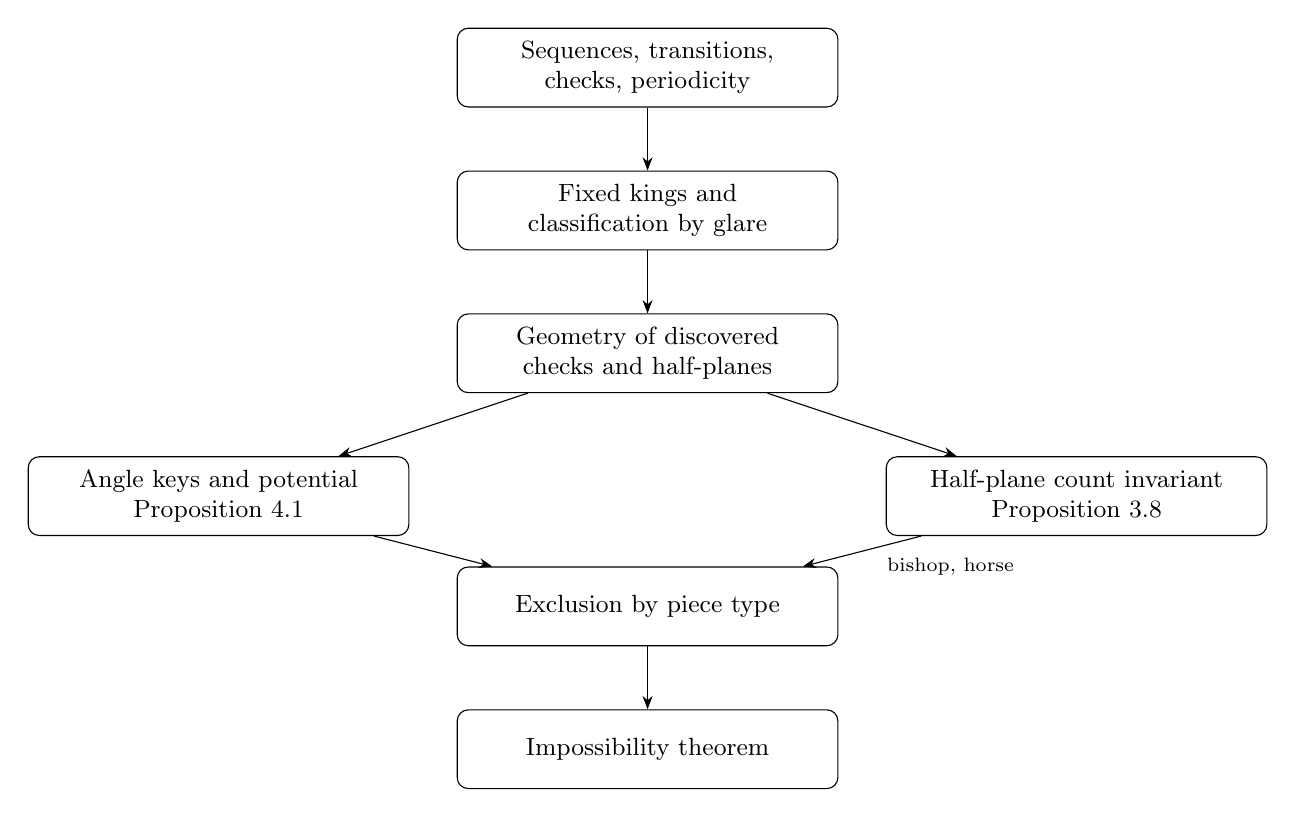
\begin{tikzpicture}[>=Stealth, every node/.style={draw,rounded corners,align=center,font=\small,text width=46mm,minimum height=10mm},node distance=8mm and 6mm]
\node (model) {Sequences, transitions, checks, periodicity};
\node (glare) [below=of model] {Fixed kings and\\classification by glare};
\node (geom) [below=of glare] {Geometry of discovered checks and half-planes};
\node (angle) [below left=of geom] {Angle keys and potential\\Proposition 4.1};
\node (count) [below right=of geom] {Half-plane count invariant\\Proposition 3.8};
\node (cases) [below=22mm of geom] {Exclusion by piece type};
\node (main) [below=of cases] {Impossibility theorem};
\draw[->] (model)--(glare);\draw[->] (glare)--(geom);
\draw[->] (geom)--(angle);\draw[->] (geom)--(count);
\draw[->] (angle)--(cases);\draw[->] (count)--node[draw=none,text width=17mm,minimum height=0pt,font=\scriptsize,below right,pos=0.4]{bishop, horse}(cases);
\draw[->] (cases)--(main);
\end{tikzpicture}
\caption{Conceptual proof dependencies for shogi; proposition numbers are those of the original paper. The path from the piece-count condition is omitted. The full import graph is in the reproduction materials.}\label{fig:proof}
\end{figure}

By Proposition 4.1 of the original paper, the first player gives a discovered check on some move.
The piece moved on that move is not a king and is non-glaring.
We use a forward potential for knights, lances and pawns, the directions of movement for gold-type pieces, and geometry and the number of bishops and rooks for silvers, rooks and dragons.
In the remaining configurations for bishops and horses, the case analysis of Table 1 of the original paper and Proposition 3.8 of the original paper contradict each other.
We also check, on the dependency paths of the proof term, that bishops and horses are the only piece types whose exclusion uses the half-plane invariant.

\section{Reconstructing the shogi proof}
\subsection{Rational angle keys}
Instead of treating the angle \(\angle AKL\) of the original paper directly through inverse trigonometric functions on the reals, we use, for \(u=A-K\) and \(v=L-K\),
\[
 f_v(u)=-\frac{(u\cdot v)|u\cdot v|}{u\cdot u}\in\mathbb Q.
\]
For nonzero vectors this equals \(-\|v\|^2\cos\theta|\cos\theta|\) mathematically.
Rather than proving a full equivalence with trigonometric functions, the implementation proves the following two properties, which the later arguments need.
\begin{enumerate}
\item The value does not change when \(u\) is scaled by a positive integer.
\item If \(u\) and \(v\) are not parallel and \(a,b>0\), then the key of \(au+bv\) is smaller than the key of \(u\).
\end{enumerate}
The value at the zero vector is also defined, but wherever the geometry is used we prove the required nonzero and non-parallel conditions.
\decl{MPC.vecKey_of_mul}
\decl{MPC.vecKey_lt_of_comb}

To prove the second property, put \(s=u\cdot v\) and \(t=(au+bv)\cdot v\).
With \(Q=u\cdot u\), \(C=(au+bv)\cdot(au+bv)\), \(V=v\cdot v\) and \(X=\det(u,v)\), we use the identity
\[
 t^2Q-s^2C=X^2(2ab\,s+b^2V)
\]
and reduce to a comparison of rationals by splitting on the signs of \(s\) and \(t\).
This makes the geometric argument of the original paper, that an interposition strictly lowers the key, available through integer and rational arithmetic.

\subsection{A potential defined on each position}\label{sec:potential}
Fix a side \(o\), let \(K\) be its king and \(L\) the opponent's king.
Let \(c_k\) be the square of the checking piece in state \(k\) and \(N_k\) the set of squares of the opponent's non-glaring pieces, and define
\[
 \Phi_o(k)=f_{L-K}(c_k-K)+\sum_{q\in N_k}f_{L-K}(q-K).
\]
The properties needed for choosing the checking piece and for its uniqueness are proved beforehand.
We do not build a map identifying individual pieces before and after a period; we sum over the actual set of squares in each state.
\decl{MPC.MoveTrace.anglePotential}

Suppose that side \(o\) never gives a discovered check.
Then \(\Phi_o\) does not change on the direct checks of that side, and does not increase on the moves of the opponent.
In a discovered check, the term of the source cancels against the term of the new checking piece.
Since the first and last values agree by periodicity, the change on every single move is 0.
The condition for equality on the opponent's moves means that the opponent captures the checking piece on every move.
The opponent's hand then grows each time and does not shrink on the moves of \(o\), which contradicts periodicity.
This holds for both sides and gives Proposition 4.1.
\decl{MPC.MoveTrace.discoveredCheckByEachSide_of_mutualPerpetualCheck}

This construction expresses the sum of Lemma 4.7 of the original paper as a quantity on positions.
The proof of Lemma 4.6 in the GPW version also takes, on each position, the sum of the angles that a player's pieces on the board not glaring at the opponent's king make at that king, and expresses the change on one move as a difference of these sums~\cite{gpw}; expressing the sum as a quantity on positions is shared with this paper.
Our potential replaces the angles by rational keys and adds a term for the checking piece.
We do not assume that an arbitrary monotone transformation preserves all the angle identities of the original paper.
The important point is that the change on each move and the cancellation are proved anew in Lean using the keys.

\subsection{Half-plane counts and balance in natural numbers}
Using the signed position \(\ell(q)\) relative to the line through the two kings, we specify for an integer \(s\) the region \(s\ell(q)>0\).
The values \(s=1,-1\) correspond to the two half-planes, and \(s=0\) to the empty region.
Squares on the boundary are not included.
Let \(O_s(k)\) be the set of squares in this region that hold a piece, do not glare at the opponent's king, and are touched by the sequence, and let \(C_s(k)\) be the set of squares of checking pieces in the same region.
Then
\[
 D_s(k)=|O_s(k)|+|C_s(k)|
\]
is \code{discHCount}.
We examine membership in the concrete sets move by move, and lift the changes at the source and the destination to equations between cardinalities of finite sets.
To avoid truncated subtraction, the balance is handled as additive equations.
The invariance under one move, proved separately for board moves and drops, is extended to all states by induction on a finite index.
\decl{MPC.MoveTrace.discHCount_succ_eq}
\decl{MPC.MoveTrace.discHCount_eq_of_periodic}

\section{Formalizing chess}\label{sec:chess}
\subsection{Model and main theorem}
Section 6 of the original paper states that the facts up to Section 4 also hold for chess, and proves the chess case through the geometry of checking rays and crossings.
In the formalization, an 8\(\times\)8 model lives in the namespace \code{MPC.Chess}, which imports no shogi declarations at all.
The facts from earlier sections that Section 6 uses are proved again on this model.

A position \code{Position} consists of the board, the side to move, four castling rights and an en-passant target square; there are no pieces in hand.
A \code{Move} is an ordinary move (which may capture or promote), an en-passant capture, or castling, and \code{applyMove} updates the board, the side to move, the rights and the target independently of legality.
\code{LegalMove} consists of the agreement of the king placement before the move, \code{PseudoLegal}, which collects the local conditions of Article 3 of the FIDE Laws, and the safety of the mover's king after the move~\cite{fide}.
\code{PseudoLegal} forbids capturing one's own pieces or a king, and covers pawn advances, captures, double steps and en passant, compulsory promotion on the last rank, and the rights, path and attacked squares of castling.
\code{FollowsLegalMoves} requires that each move be such a legal move for some king placement and that the next state be given by \code{applyMove}.
As for shogi, attack \code{attacks} is separated from check \code{inCheck}, and pinned pieces still attack.

\begin{theorem}[Formalization of the theorem of Section 6 of the original paper]
There is no finite move sequence of positive length with a sequence of king squares in which every move is legal (\code{FollowsLegalMoves}), the king placement agrees in every state (\code{KingsWellPlaced}), every move checks the opponent's king (\code{EveryMoveChecksOpponent}), and the final board and side to move equal the initial ones (\code{BoardTurnPeriodic}).
\end{theorem}
\decl{MPC.Chess.mutual_perpetual_check_impossible}

The main theorem requires only the board and the side to move to recur.
Our model of repetition under Article 9.2.3 of the FIDE Laws, \code{FIDESamePosition}, also compares each player's retained castling rights and the legal moves available to the side to move.
Losing a castling right distinguishes positions even when the path is blocked (Article 9.2.3.2).
Once the board, turn and rights agree, only a difference in which en-passant captures are legal can distinguish the positions (Article 9.2.3.1).
A return to the initial position in this sense would repeat its board and turn, so the main theorem rules it out.
\decl{MPC.Chess.mutual_perpetual_check_impossible_of_fideSamePosition}
Reachability from the initial position, draw claims by repetition, threefold and fivefold repetition, the 50- and 75-move rules and clocks are not among the premises.
A sequence of length 0 can satisfy all the other conditions, so the condition of positive length cannot be dropped.
The bound on bishops and rooks from shogi is not carried over, and the number of promoted pieces is not limited.

\subsection{Reductions by periodicity and the facts of Sections 2 and 3}
The original paper argues that the sequence contains no captures because captured pieces cannot be dropped.
In the formalization, the number of pieces on the board, the number of pawns and the total advance of the pawns are defined as weighted sums over the board.
The number of pieces strictly decreases on a capture and the number of pawns on a promotion, and among the remaining moves the total advance strictly increases when a pawn moves.
By the periodicity of the board these quantities are equal in all states, which rules out, in turn, captures, en passant, promotions and pawn moves.
\decl{MPC.Chess.MoveTrace.pieceCount_eq_of_periodic}
In a periodic mutual check of positive length the side to move is in check in every state, so castling, which requires not being in check at the start, does not occur either.
\decl{MPC.Chess.MoveTrace.not_castle_of_periodic_checks}

The immobility of the kings (Proposition 2.2) follows because a king move breaks the alignment of the two kings, and moves other than king moves cannot restore it.
A checking piece is neither moved nor captured by the reply, so a check by a pawn or a knight, which does not depend on intermediate squares, would remain after the reply and violate the safety of the replying king.
Checking pieces are therefore limited to queens, rooks and bishops.
\decl{MPC.Chess.MoveTrace.kingPositions_eq_of_periodic_checks}
\decl{MPC.Chess.MoveTrace.checking_piece_is_slider_of_periodic_checks}
The classification by glare (Lemmas 2.4--2.6 and 2.8), the persistence of the lines of discovered checks (Proposition 3.3 and Corollary 3.4), and the exclusion of landings and checks on the line through the two kings (Propositions 3.5 and 3.6) are also proved on this model without identifying individual pieces.
Since there are no captures, the destination in Corollary 3.4 lies strictly inside both lines.

\subsection{Checking rays and crossings}
A half-line from a king in one of the eight queen directions is a checking ray \code{CheckingRay} (Definition 6.1) if, in some state, an opponent's piece on it actually checks this king.
We prove Lemma 6.2, whose proof the original paper omits and the GPW version gives~\cite{gpw}: every move goes between two different checking rays, for each of the two kings.
The proof splits into checks from the destination, checks by unblocking, and the next departure.
\decl{MPC.Chess.MoveTrace.every_move_between_distinct_checkingRays}

Crossings (Definition 6.3) need not be squares of the board, so we extend the half-lines to rational coordinates \(\mathbb Q^2\) and prove that the computation of intersections by determinants is equivalent to membership in both half-lines.
The parallel case is handled by a separate classification theorem, and Proposition 3.5 rules out parallel overlaps of checking rays.
From the pairs of directions of the two kings we build the finite set of crossings (at most 64 points) and sort the points on each half-line by their parameter.
A1 and A2 are defined with proofs that the half-line contains at least one and at least two points, respectively, as arguments; no default value is filled in.
From the conditions on the sequence, including the required counts, we derive Lemma 6.4(1), that a checking piece is at A2 or farther, and Lemma 6.4(2), that a checking piece at A2 moves at some point in the sequence.
\decl{MPC.Chess.MoveTrace.checker_eq_or_beyond_second_of_periodic_checks}
\decl{MPC.Chess.MoveTrace.checker_at_second_departs_of_periodic_checks}

\subsection{Angle ranks and the candidates of Figure 3}
The angles of Definition 6.5 are not computed as real angles; using the inner and cross products with the displacement to the other king, we classify them into ranks 1--4 for \((0^\circ,45^\circ]\), \((45^\circ,90^\circ]\), \((90^\circ,135^\circ]\) and \((135^\circ,180^\circ)\).
We prove the triangle argument that if non-parallel half-lines from the two kings intersect, the sum of their ranks is at most 4, and together with Lemma 6.4(1) we derive that every checking ray has rank at most 2.
\decl{MPC.Chess.kingRayRank_add_le_four}
\decl{MPC.Chess.MoveTrace.checkingRay_rank_le_two_of_periodic_checks}

The original paper counts the candidates up to translation, rotation and reflection.
We express this by putting one king at the origin and by the eight symmetries of the lattice, \code{LatticeFrame}, made of swapping the coordinates and changing their signs.
With the king \(K\) at the origin and the other king \(L\) at canonical coordinates \((a,b)\) with \(0\le b\le a\) and \(0<a\), the two rays of rank 2 are parallel and do not meet when \(b=0\) or \(b=a\).
When \(0<b<a\), the checking rays on one half-plane are the northeast and north rays from \(K\) and the west and northwest rays from \(L\).
Since the four crossings \((b,b)\), \(((a+b)/2,(a+b)/2)\), \((0,b)\) and \((0,a+b)\) are squares of the board, \((a,b)\) is one of \((3,1)\), \((5,1)\) and \((4,2)\).
If the opposite half-plane also has checking rays, only \((3,1)\) remains (Figure~\ref{fig:figure3}).
\decl{MPC.Chess.MoveTrace.figure3_candidates_of_periodic_checks}

\begin{figure}[ht]
\centering
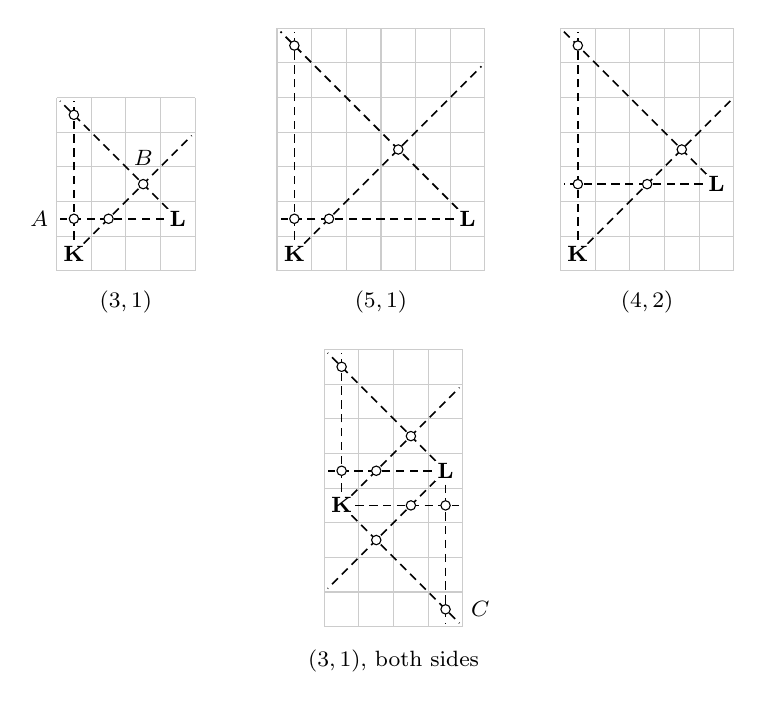
\begin{tikzpicture}[x=4.4mm,y=4.4mm,
  grd/.style={gray!40,step=1},
  ray/.style={densely dashed,semithick},
  pt/.style={circle,draw,fill=white,inner sep=1.2pt},
  kg/.style={font=\footnotesize\bfseries,fill=white,inner sep=0.8pt},
  lab/.style={font=\footnotesize,inner sep=1pt}]
\begin{scope}
\draw[grd,shift={(-0.5,-0.5)}] (0,0) grid (4,5);
\draw[ray] (0,0)--(3.4,3.4); \draw[ray] (0,0)--(0,4.4);
\draw[ray] (3,1)--(-0.4,1); \draw[ray] (3,1)--(-0.4,4.4);
\foreach \p in {(1,1),(2,2),(0,1),(0,4)} \node[pt] at \p {};
\node[kg] at (0,0) {K}; \node[kg] at (3,1) {L};
\node[lab] at (-1,1) {\(A\)}; \node[lab] at (2,2.75) {\(B\)};
\node[font=\footnotesize] at (1.5,-1.4) {\((3,1)\)};
\end{scope}
\begin{scope}[xshift=28mm]
\draw[grd,shift={(-0.5,-0.5)}] (0,0) grid (6,7);
\draw[ray] (0,0)--(5.4,5.4); \draw[ray] (0,0)--(0,6.4);
\draw[ray] (5,1)--(-0.4,1); \draw[ray] (5,1)--(-0.4,6.4);
\foreach \p in {(1,1),(3,3),(0,1),(0,6)} \node[pt] at \p {};
\node[kg] at (0,0) {K}; \node[kg] at (5,1) {L};
\node[font=\footnotesize] at (2.5,-1.4) {\((5,1)\)};
\end{scope}
\begin{scope}[xshift=64mm]
\draw[grd,shift={(-0.5,-0.5)}] (0,0) grid (5,7);
\draw[ray] (0,0)--(4.4,4.4); \draw[ray] (0,0)--(0,6.4);
\draw[ray] (4,2)--(-0.4,2); \draw[ray] (4,2)--(-0.4,6.4);
\foreach \p in {(2,2),(3,3),(0,2),(0,6)} \node[pt] at \p {};
\node[kg] at (0,0) {K}; \node[kg] at (4,2) {L};
\node[font=\footnotesize] at (2,-1.4) {\((4,2)\)};
\end{scope}
\begin{scope}[xshift=34mm,yshift=-32mm]
\draw[grd,shift={(-0.5,-3.5)}] (0,0) grid (4,8);
\draw[ray] (0,0)--(3.4,3.4); \draw[ray] (0,0)--(0,4.4);
\draw[ray] (3,1)--(-0.4,1); \draw[ray] (3,1)--(-0.4,4.4);
\draw[ray] (0,0)--(3.4,0); \draw[ray] (0,0)--(3.4,-3.4);
\draw[ray] (3,1)--(3,-3.4); \draw[ray] (3,1)--(-0.4,-2.4);
\foreach \p in {(1,1),(2,2),(0,1),(0,4),(3,0),(2,0),(3,-3),(1,-1)} \node[pt] at \p {};
\node[kg] at (0,0) {K}; \node[kg] at (3,1) {L};
\node[lab] at (4,-3) {\(C\)};
\node[font=\footnotesize] at (1.5,-4.5) {\((3,1)\), both sides};
\end{scope}
\end{tikzpicture}
\caption{The four candidates of Figure 3 of the original paper, drawn in the canonical coordinates of this formalization (our own drawing). \(K\) is at the origin, \(L\) at \((a,b)\), and north is up. Dashed lines are checking rays and white circles are crossings; the extent of the board is not shown. The top row has checking rays on one half-plane only, the bottom row on both.}\label{fig:figure3}
\end{figure}

For the three upper candidates, since the displacement of every move is a straight line or a knight's move, Lemma 6.2 leaves only moves between \(A\) and \(B\) in \((3,1)\).
If every move goes between two squares, the colour of the piece moved first disagrees with the side to move next.
For the lower candidate, the crossings on the half-line south from \(L\) are the two points \((3,0)\) and \(C\), so A2 is \(C\).
By the distances on the board, the checking piece on this half-line is at \(C\), and by Lemma 6.4(2) it departs from \(C\), but no destination satisfies both the condition of Lemma 6.2 and the movement condition of the piece.
\decl{MPC.Chess.MoveTrace.false_of_upper_candidate}
\decl{MPC.Chess.MoveTrace.false_of_lower_candidate}

\subsection{Differences from the original paper}
Section 6 of the original paper (third edition) refers to the facts up to Section 4 as holding ``in the same way'', and omits the proof of Lemma 6.2 and the enumeration of the candidates of Figure 3.
The GPW version gives a proof of Lemma 6.2~\cite{gpw}.
The formalization gives all of these as theorems.
The exclusion of captures is derived from the monotonicity of the piece count and periodicity, and the exclusion of promotion, en passant and castling is made explicit.
Crossings are handled in rational coordinates, and parallel half-lines are separated from the non-parallel computation.
Angles are replaced by ranks and rotations and reflections by lattice symmetries; no real trigonometric functions are used.
These are independent proofs for the chess model and share no lemmas with the shogi proof.

\section{Verification materials and proof engineering}
\subsection{Verification method}
We use Lean 4.36.0 and a pinned Mathlib revision.
The result of \texttt{\#print axioms} for each of the two main theorems, for shogi and chess, consists only of \code{propext}, \code{Classical.choice} and \code{Quot.sound}.
These are Lean's standard logical foundations, not axioms about shogi or chess introduced by this project.
There is no dependence on \code{sorryAx} or on additional axioms trusting native computation.
However, this result does not by itself imply that the specifications coincide with the real rules of shogi and chess.

We match the type of the shogi main theorem concretely, and check that Proposition 4.1, the bound on piece counts in every state, and the emptiness of drop squares are not additional premises.
The axiom dependencies of intermediate theorems are pinned by \texttt{\#guard\_msgs}.
Concrete examples cover the directions of both owners, blocking, king moves, promotion, capture of promoted pieces, drops and length 0.
These do not replace the theorems; they are regression checks that confirm the intended specification.

The chess verification entry point \code{MPC.Chess.Verification} checks that no shogi declaration enters the environment, and pins the axiom dependencies of the 289 public chess theorems with \texttt{\#guard\_msgs}.
It also matches the exact types of the main theorem and its corollary.
The regression examples include pawns of both colours, all directions of knights and queens, captures, double steps, promotion, en passant and castling, the rejection of moves that expose one's own king, and knight moves in a legal periodic sequence that does not keep giving check.

The two main theorems and the chess corollary are also exported together with every declaration they depend on, including Lean core and Mathlib, and type-checked from an empty environment by nanoda 0.4.17, a type checker that ships with Lean but is implemented separately from Lean's kernel.
Only the three axioms above are permitted; any other axiom makes the check fail.
As negative controls, every run also confirms that nanoda rejects a false proof added with the kernel's type check switched off, and a theorem that derives a contradiction from an extra axiom.
In addition, leanchecker, which also ships with Lean, replayed the declarations of every module of this project through the kernel, in an environment that loads only the imports of that module, and all of them passed.
This check detects declarations that entered the environment without passing the kernel's type check; it is not independent of Lean's kernel.
The nanoda check is part of the whole verification, while the leanchecker replay, which takes about 7 minutes, is run separately.

\IfFileExists{metrics_en.tex}{% Generated by scripts/paper_metrics.py. Do not edit.
\begin{table}[ht]\centering\small
\begin{tabular}{lrrrr}\toprule
Category & Files & Code lines & Comment-only lines & Blank lines\\\midrule
Shogi: proof & 58 & 9382 & 1693 & 825\\
Shogi: verification and audit & 54 & 6818 & 1455 & 952\\
Shogi: legacy API & 8 & 247 & 66 & 37\\
Chess: proof & 40 & 5478 & 449 & 638\\
Chess: verification & 22 & 2803 & 636 & 707\\
\bottomrule\end{tabular}
\caption{Physical line counts. A line containing both code and a comment counts as a code line.}
\end{table}
Configuration, scripts, documents and Mathlib are not counted.
We do not use the size of the proof as a measure of novelty or of the strength of verification.
Using caches of the pinned dependencies, we re-ran the whole verification in a separate
directory without any build products of this project, in 202.0 seconds (a single measurement).
The environment, conditions and logs are recorded in the reproduction materials.
}{See the accompanying reproduction materials for the verification statistics.}

\subsection{Code organization and compatibility}
The shogi proof is divided into foundations, sequences, glare, geometry, invariants and piece-specific arguments.
Reading the main theorem does not require following the Part numbers of the development order.
The old direction predicates and compatibility theorems are isolated in a Legacy layer and excluded from the import closure of the main proof.
The verification modules are detached from the aggregate import of the proof and built as a separate target.
The chess formalization under \code{MPC.Chess} is a separate build target, and no shogi module imports \code{MPC.Chess}.

Public declaration names are kept in principle, and a table of module moves is provided.
Lemmas duplicated in several files, such as player flipping, are collected in the foundations layer.
The comment cleanup removes no code; it moves the historical ledger of axioms into documents.
Comments on mathematical meaning, assumptions and proof intent are kept, as are the expected-output comments used in verification.

\subsection{Distinguishing AI assistance from audit}
The development history records proof and implementation work done with AI assistance, and AI assistance was also used in organizing this paper and in writing its first draft.
This English version was likewise produced from the Japanese manuscript with AI assistance.
We distinguish the research subject and the scope of the cleanup, chosen by a human, from the proof candidates and text generated by AI.
What the kernel checks is the proof term, not the author's originality, the citations or the adequacy of the specification.
Because we have not reproducibly measured past human working time or AI success rates, we make no numerical claims about them.
This paper is a first research draft, and it will be published only on GitHub after the author's final review of its content.

\subsection{Published materials}
The TeX sources and PDFs of this paper, the Lean source code, the verification records and the instructions for reproduction are published at \url{https://github.com/funaken/mutual-perpetual-check-lean}.
The text and figures are provided under CC0 1.0 and the source code under MIT-0. The PDF of the original paper is not included.

\section{Related work, limitations and future work}\label{sec:related}
As a natural-language argument for the same theorem, Fernando published on Chess Stack Exchange on January 14, 2022 an argument that, with ordinary pieces, there is no cycle in which both players give check on every move~\cite{fernando}.
The argument rules out captures, pawn moves and castling in a cycle, and shows that the kings do not move.
Next, since the number of pieces lined up with the enemy king in their direction of attack, ignoring the pieces in between, does not decrease, it restricts the source and destination of every move to squares in line with each of the two kings.
It then lists the possible moves for the relative positions of the kings, separated into orthogonal, diagonal and unaligned cases, and excludes a cycle with a lemma that the half-line from a king through a square must carry at least two moving pieces.
It claims to hold even on an infinite board, and only the results of the case analysis for knight moves are given.
Our formalization of chess follows Nanka's proof and does not formalize Fernando's argument, but it contains stages comparable to it: Proposition 2.2 of the original paper (the immobility of the kings), Lemma 6.2, and the enumeration of the candidates of Figure 3.
For shogi, the GPW version reports that partial arguments, such as the immobility of the kings, were published in 2008, and that they do not complete a proof on their own~\cite{gpw}.
As for formalizations of the same theorem in a proof assistant, we found none within the scope of our survey, as stated in Section 1.

Hurd verified endgame tables using HOL4 and BDDs~\cite{hurd}, and Marić et al.\ proved a KRK endgame strategy with Isabelle/HOL and Z3~\cite{krk}.
This work does not target a specific endgame strategy or a precomputed table of positions; it excludes the existence of periodic sequences using geometry and invariants.
Yamaoka's \code{lean-shogi} shows agreement between position-wise legal-move generation and a specification, but leaves history-dependent repetition out of scope~\cite{yam}.
The two are complementary, and because their representations of coordinates and transitions differ, neither can be reused automatically in the other.

This work has three limitations.
First, there is no formal inclusion theorem connecting the complete legal-move relation of ordinary shogi to this model.
Second, the local legal moves of chess follow the FIDE Laws, but we have proved neither reachability from the standard initial position nor agreement with another formalization of chess.
Third, we have not experimentally evaluated whether the techniques of this formalization are effective in other large proofs.
Future work includes connecting to a separate rules model, unifying and reusing the lemmas on glare, geometry and periodicity that shogi and chess duplicate, and third-party review of the specification.

What this paper presents is a kernel-checkable proof of a known impossibility theorem with its assumptions made explicit, together with the reconstruction that the formalization required.
The survey log on novelty, the table mapping propositions to declarations, the comparison of types and axiom dependencies, and the commands for reproduction are provided with the code.

\begin{thebibliography}{9}
\bibitem{nanka}Nanka (なんか). 将棋およびチェスにおいて双方連続王手の千日手が成立しないことの証明 [A proof that mutual perpetual check cannot occur in shogi and chess; in Japanese]. 3rd edition, March 9, 2024. This formalization is based on that PDF. Background of the publication: \url{https://yaneuraou.yaneu.com/2024/03/03/proof-of-the-impossibility-of-perpetual-check-in-shogi/}.
\bibitem{gpw}Masanari Shimura (志村将也). 双方連続王手による同一局面反復の不可能性について [Impossibility of Repetition by Mutual Perpetual Check; in Japanese]. In: The 31st Game Programming Workshop (GPW 2026), pp.~85--92. Information Processing Society of Japan, November 2026. Presentation 5-2: \url{https://www.gi-ipsj.org/gpw/2026/program.html}.
\bibitem{fernando}Ravi Fernando. Answer to ``Infinite sequence of consecutive checks allowing more pieces (say 9+ queens)''. Chess Stack Exchange, January 14, 2022 (edited the same day). \url{https://chess.stackexchange.com/a/38960}. Accessed November 28, 2026.
\bibitem{hurd}Joe Hurd. Formal Verification of Chess Endgame Databases. 2005. \url{https://gilith.com/papers/chess.pdf}.
\bibitem{krk}Filip Marić, Predrag Janičić, Marko Maliković. Proving Correctness of a KRK Chess Endgame Strategy by using Isabelle/HOL and Z3. CADE, 2015. \url{https://poincare.matf.bg.ac.rs/~janicic/papers/2015-cade-krk.pdf}.
\bibitem{yam}Tadao Yamaoka. lean-shogi. 2026. Commit consulted: \nolinkurl{2610d0f8af31cf94d612b71c27f4696ba3691d51}. \url{https://github.com/TadaoYamaoka/lean-shogi}.
\bibitem{rules}Japan Shogi Association. 対局規則 [Rules of play], Articles 4, 5, 8 and 10. \url{https://www.shogi.or.jp/match/taikyoku_rules/}. Accessed November 8, 2026.
\bibitem{fide}FIDE. FIDE Laws of Chess, taking effect from 1 January 2023. Articles 3 and 9.2.3. \url{https://handbook.fide.com/chapter/e012023}. Accessed November 23, 2026.
\end{thebibliography}
\end{document}
